%\DefineVerbatimEnvironment{code}{Verbatim}{frame=single,rulecolor=\color{blue}}
\newcommand{\mathbfx}[1]{{\mbox{\boldmath $#1$}}}
\renewcommand{\P}{{\mathbb P}}
\renewcommand{\H}{{\mathbb H}}
\newcommand{\GG}{\mathbf{G}}
\newcommand{\kentc}[1]{\marginpar{\tiny KAM: #1}}
\newcommand{\rckc}[1]{\marginpar{\tiny RCK: #1}}

\fenicschapter{Constructing general reference finite elements}
              {Constructing general reference finite elements}
              {Robert C. Kirby and Kent-Andre Mardal}
              {kirby-1}

%\begin{document}

%\maketitle
%\vspace{-0.3cm}

\thispagestyle{empty}

%\editornote{Reuse color figures from chapter [kirby-7] for RT elements etc.}

This chapter describes the mathematical framework for constructing a
general class finite elements on 
reference domains. This framework is used by both the FIAT and SyFi
projects, see the Chapters~\ref{chap:kirby-2} and ~\ref{chap:alnes-3}, respectively.  
Our goal is to provide a framework by which simplicial finite elements
with very complicated bases can be constructed automatically.  We work from the classic Ciarlet definition of the finite
element and its ``nodal'' basis (an abstract notion far more general
and powerful than standard node-oriented Lagrange polynomials).  

To date, our methodology does not include spline-type spaces such as
are becoming widely popular in isogeometric analysis~\citep{HughesCottrellBazilevs2005}, nor does
it entirely address XFEM~\citep{ChessaSmolinskiBelytschko2002} or {\em hp}-type methods~\citep{Schwab1998}.  However, in isogeometric
analysis, the basis functions are readily defined by simple recurrence
relations from from the theory of splines, so a tool like FIAT or SyFi
is not necessary.  XFEM typically works by enriching existing
finite element spaces with special basis functions to capture singular
behavior -- our approach can provide the regular basis but not the
``extra'' functions.  Finally, handling the constraints imposed in
$hp$ methods is possible, but unwieldy, with our methodology, but
tetrahedral $hp$ bases are available~\citep{AinsworthCoyle2003}.  We
return to some of these issues later.

\section{Background}
The finite element literature contains a huge collection of
approximating spaces and degrees of freedom, many of which are
surveyed in Chapter~\ref{chap:kirby-6}.
Some applications, such as Cahn-Hilliard and
other fourth-order problems, can benefit from very smooth finite
element bases,  while porous media flow requires
vector fields discretized by piecewise polynomial functions with
only normal components continuous across cell boundaries.  Many problems in
electromagnetism call for the tangentially continuous vector fields obtained
by using \nedelec\ elements~\citep{Nedelec1980,Nedelec1986}.  Many elements are carefully designed
to satisfy a \emph{inf-sup} condition~\citep{BrezziFortin1991,GiraultRaviart1986},
originally developed to explain stability of discretizations of
incompressible flow problems.  Additionally, some problems call for low-order
discretizations, while others are effectively solved with high-order
polynomials.

While the automatic generation of computer programs for finite element
methods requires one to confront the panoply of  finite
element families found in the literature, it also provides a pathway
for wider employment of Raviart--Thomas, \nedelec, and other
difficult-to-program elements.
Ideally, one would like to
describe the diverse finite element spaces at an abstract level,
whence a computer code discerns how to evaluate and differentiate
their basis functions.  Such goals are in large part accomplished by
the FIAT and SyFi projects, whose implementations are described in
later chapters.

Projects like FIAT and SyFi may ultimately remain
mysterious to the end user of a
finite element system, as
interactions with finite element bases are typically mediated through
tools that construct the global finite element operators.
The end user will typically be satisfied if two conditions are met.
First, a finite element system
should support the common elements used in the application
area of interest.  Second, it should provide flexibility with respect
to order of approximation.

It is entirely possible to satisfy many users by \emph{a priori}
enumerating a list of finite elements and implement only those.  At certain times, this
would even seem ideal.  For example, after the rash of research
that led to elements such as the Raviart--Thomas-\nedelec\ and
Brezzi-Douglas-Marini families, development of new families slowed
considerably.  Then, more recent work lead forth by  Arnold, Falk, and Winther in the context of exterior
calculus has not only led to
improved understanding of existing element families, but has also
brought a new wave of elements with improved properties.  A
generative system for finite element bases can far more
readily assimilate these and future developments.
Automation also provides generality with respect to the order of approximation that standard libraries
might not otherwise provide. Finally, the end-user might even easily define his own new element
and test its numerical properties before analyzing it mathematically.


In the present chapter, we describe the mathematical formulation
underlying such projects as FIAT, SyFi and Exterior~\citep{LoggMardal2009}.
This formulation starts from definitions of finite elements as
given classically by Ciarlet~\citep{Ciarlet2002}.  It then uses basic linear
algebra to construct the appropriate basis for an abstract
finite element in terms of polynomials that are easy to implement and
well-behaved in floating point arithmetic.  We focus on
constructing nodal bases for a single, fixed reference element.  As we
will see in the Chapters~\ref{chap:alnes-3} and ~\ref{chap:logg-1}, form compilers such as
\texttt{ffc} and \texttt{sfc} will work
in terms of this single reference element.


Other approaches exist in the literature, such as the hierarchical
bases studied by Szabo and Babuska~\citep{SzaboBabuska1991} and extended to \(
\Hcurl \) and \( \Hdiv \) spaces in work such
as~\citep{AinsworthCoyle2003}.  These approaches can provide greater flexibility for
refining the mesh and polynomial degree in finite element methods, but
they also require more care during assembly and are typically constructed
on a case-by-case basis for each element family.  When they are
available, they may be cheaper to construct than using the technique
studied here, but this present technique is easier to apply to an
``arbitrary'' finite element and so is considered in the context of
automatic software.


\section{Preliminaries}
Both FIAT and SyFi work with a slightly modified version of the  abstract definition of a finite element introduced by
Ciarlet.
\begin{definition}[Finite element~{\citep{Ciarlet2002}}]
  A finite element is defined by a triple
  $(T, \CiarletSpace,\mathcal{L})$, where
  \femdefinition{}
  \label{chap:kirby-1:fedef} 
\end{definition}
In this definition, the term ``finite element'' refers not only to
a particular cell in a  mesh, but also to the associated function
space and degrees of freedom.  Typically, the domain \( T \) is some
simple polygonal or polyhedral shape and the function space \( \mathcal{V} \)
consists of polynomials.

Given a finite element, a concrete
basis, often called the nodal basis,
for this element can be computed by using the following definition.

%The function space \( P \)
%typically consists of polynomials.  Also, this definition is
%slightly more general than Ciarlet's in that the range of the
%functions could be a space of vectors or tensors.  Thus, the extended
%definition captures things like Raviart-Thomas and Arnold-Winther
%elements.


\begin{definition}
The \emph{nodal basis} for a finite element \( (T,\mathcal{V},\mathcal{L}) \) 
is the set of functions \( \{ \phi_i \}_{i=1}^{n} \) such
that for all \( 1 \leq i,j \leq n \),
\begin{equation}
l_i(\phi_j) = \delta_{ij}.
\end{equation}
\label{chap:kirby-1:nodaldef}
\end{definition}

The main issue at hand in this chapter is the \emph{construction} of
this nodal basis.  For
any given finite element, one may construct the nodal basis
explicitly with elementary algebra.  However, this becomes tedious as
we consider many different families of elements and want arbitrary
order instances of each family.  Hence, we present a new 
paradigm here that undergirds computer programs for automating the
construction of nodal bases.

In addition to the construction of the nodal base we need to keep in mind that
finite elements are patched together to form a piecewise
polynomial field over a mesh. The fitness (or stability) of a particular finite element method for a particular problem relies on the continuity
requirements of the problem. The degrees of freedom of a particular element
are often chosen such that these continuity requirements are fulfilled.

Hence, in addition to computing the nodal basis, the framework developed here
simplifies software for the following tasks:

\begin{enumerate}
\item Evaluate the basis functions and their derivatives at points.
\item Associate the basis functions (or degree of freedom) with
      topological facets of \( K \) such as its vertices, edges and its
      placement on the edges.
\item Associate each basis function with additional meta-data that describes  
      the mapping that should be used for the evaluation of the basis functions and their derivatives.
\item Provide rules for evaluating the degrees of freedom applied to arbitrary functions 
      (needed for Dirichlet boundary conditions).
\end{enumerate}


The first of these is relatively simple in the framework
of symbolic computation (SyFi), but they require more care if an
implementation uses numerical arithmetic (FIAT).  The middle two
encode the necessary information for a client code to transform the
reference basis and assemble global degrees of freedom when the
finite element is either less or more than $C^0$ continuous. The final
task may take the form of a point at which data is evaluated or
differentiated or more generally as the form of a sum over points and
weights,  much like a quadrature rule.

%\kentc{Link this to the appropriate discussion in form/FFC/SFC chapters }

\section{Mathematical framework}
\subsection{Change of basis}

%\editornote{Coordinate with notation in Chapter~\ref{chap:kirby-7} where $B$ is used for the Vandermonde matrix.
%Perhaps we could use $\mathcal{V}$? Also use $\ell$ for the functionals and $\alpha$ for the expansion coefficients.}

The fundamental idea in constructing nodal basis is from elementary
linear algebra: one constructs the desired (nodal) basis as a linear
combination of another available basis.  We will start with some
basis \( \left\{ \psi_i \right\}_{i=1}^{n} \mbox{that spans} \  \mathcal{V}  \).  From
this, we construct each nodal basis function $\phi_j$ as
\begin{equation}
 \phi_j = \sum_{k=1}^n \alpha_{jk} \psi_k,
\end{equation}
The task is to compute the matrix \( \alpha \).  Each fixed \( \phi_j \) must
satisfy
\begin{equation}
\ell_i( \phi_j ) = \delta_{ij},
\end{equation}
and using the above expansion for \( \phi_j \), we obtain
\begin{equation}
\delta_{ij} = \sum_{k=1}^n \ell_i( \alpha_{jk} \psi_{k} ) = \sum_{k=1}^n \alpha_{jk} \ell_i (\psi_k).
\end{equation}
So, for a fixed \( j \), we have a system of \( n \) equations
\begin{equation}
\label{eq:singlebfA}
\sum_{k=1}^n B_{ik} \alpha_{jk} = \delta_{ij},
\end{equation}
where
\begin{equation}
B_{ik} = \ell_i(\psi_k)
\end{equation}
is a kind of generalized Vandermonde matrix.   Of course, (\ref{eq:singlebfA}) can be 
written as
\begin{equation}
B \alpha^T = I,
\end{equation}
and we obtain 
\begin{equation}
\alpha = B^{-T}.
\end{equation}
In practice, this supposes that one has an implementation of
the original basis for which the actions of the degrees of freedom  may be readily computed.
The degrees of freedom typically involves point evaluation, differentiation, integration, and so on. 


\subsection{Polynomial spaces}
In Definition \ref{chap:kirby-1:fedef} we defined the finite element in terms
of a finite dimensional function space $\mathcal{V}$. Although it is not strictly
necessary,
the functions used in finite elements are typically polynomials.
While our general strategy will in principle accommodate non-polynomial bases, we
only deal with polynomials in this chapter.
The most common space is
$\P_q^d$, the space of polynomials of degree $q$ in $\R^d$. There
are many different ways to represent $\P^d_q$. We will discuss the power
and Bernstein bases, and orthogonal bases such as Dubiner, Jacobi, and Legendre.  Each of these bases
has explicit representations or recurrence relations making them easy to 
evaluate and differentiate. In contrast,  
most finite element bases are determined by solving 
the linear system in Definition \ref{chap:kirby-1:nodaldef}.
In addition to $\P^d_q$ we will also for some
elements need $\H^d_q$, the space of homogeneous polynomials of degree
\( q \) in \( d \) variables.

Typically, the techniques developed  here
are used on simplices, where polynomials do not have a nice
tensor-product structure.  
%Some rectangular elements like the
%Brezzi-Douglas-Marini family~\citep{BrezziDouglasMarini1985a}, however, are not based on
%tensor-product polynomial spaces, and the techniques described
%in this chapter apply in that
%case as well.  
SyFi does, however, have support for rectangular domains, while  FIAT does not.

\paragraph{Power basis.}
On a line segment, the monomial or power basis 
\( \{ x^i \}_{i=0}^{q} \) spans  $\P^1_q$,  so that any \( \psi \in \P^1_q \) can be written as
\begin{equation}
\label{pn1d}
\psi = a_0 + a_1 x + \ldots a_q x^q = \sum^q_{i=0} a_i x^i.
\end{equation}
In 2D on triangles, $\P_q$ is spanned by functions on the form
\( \{ x^i y^j \}_{i,j=0}^{i+j\leq q} \), with a similar definition in
three dimensions.

This basis is quite easy to evaluate, differentiate, and
integrate. But the basis is very ill-conditioned in numerical calculations.
For instance, the condition number of the mass matrix using
the power basis in $\P^1_{10}$ gives a condition number of $5\cdot10^{14}$, 
while corresponding condition numbers are $4\cdot 10^6$ and $2\cdot 10^3$ 
for the Bernstein and Lagrange polynomials, respectively.    

\paragraph{Legendre basis.}

A popular polynomial basis for polygons that are either intervals, rectangles or boxes are the Legendre polynomials.
This polynomial basis is also usable to represent polynomials of high degree.
The basis is defined on the interval $[-1,1]$, as
\begin{equation}
\psi_i(x) = \frac{1}{2^i i!} \frac{d^i}{dx^i} (x^2 -1)^i, \quad i=0,1,\ldots,
\end{equation}
A nice feature with these polynomials is that they are orthogonal
with respect to the $L_2$ inner product, i.e.,
\begin{equation}
\int_{-1}^1 \psi_i (x) \psi_j(x) \, dx  =
\left\{
\begin{array}{c}
\frac{2}{2i+1}, \ i=j, \\
0 , \ \ i\not= j, \\
\end{array}
\right.
\end{equation}
The Legendre polynomials can be extended to rectangular domains in any dimensions by tensor--products. 
For instance, in 2D the basis reads, 
\begin{equation}
\psi_{ij}(x,y) = \psi_i(x) \psi_j(y) ,   \quad i,j \leq q. 
\end{equation}
Recurrence relations for these polynomials can be found in \citet{KarniadakisSherwin2005}.  

\paragraph{Jacobi basis.}
The Jacobi polynomials $P^{\alpha,\beta}_i(x)$ generalize the Legendre
polynomials, giving orthogonality with respect to a weighted inner
product.  In particular, $\int_{-1}^1 (1-x)^\alpha (1+x)^\beta
P^{\alpha,\beta}_i P^{\alpha,\beta}_j \, dx = 0$ unless $i=j$.  The
polynomials are given by
\begin{equation}
\label{eq:firsttwojacobi}
\begin{split}
P_0^{\alpha,\beta} & = 1 \\
P_1^{\alpha,\beta} & 
= \frac{1}{2}\left( \alpha - \beta + \left( \alpha + \beta + 2 \right)
x \right),
\end{split}
\end{equation}
with a three-term recurrence for $i\geq2$:
\begin{equation}
\label{eq:recur}
P_{i+1}^{\alpha,\beta}(x) 
= (a^{\alpha,\beta}_i x + b^{\alpha,\beta}_i) P_i^{\alpha,\beta}(x) - c^{\alpha,\beta}_i P_{i-1}^{\alpha,\beta}(x),
\end{equation}
General Jacobi polynomials are used in 1d and tensor-product domains
far less frequently than Legendre polynomials, but they play an
important role in constructing orthogonal bases on the simplex, to
which we now turn.


\paragraph{Dubiner basis.}

Orthogonal polynomials in simplicial domains are also known, although
they lack some of the rotational symmetry of the Legendre polynomials.
The Dubiner basis, frequently used in simplicial spectral
elements~\citep{Dubiner1991}, is known under many names in the literature.  It is
an \( L^2 \)-orthogonal basis that can be constructed by mapping particular
tensor products of Jacobi polynomials on a square by a singular
coordinate change to a fixed triangle.
Let \( P^{\alpha,\beta}_n \) denote the \( n^\mathrm{th} \) Jacobi
polynomial with weights \( \alpha, \beta \).  Then, define the
new coordinates
\begin{equation}
\label{eq:dubcoord}
\begin{split}
\eta_1 & = 2\left(\frac{1+x}{1-y}\right)-1 \\
\eta_2 & = y,
\end{split}
\end{equation}
which map the square \( [-1,1]^2 \) to the triangle with
vertices \( (-1,-1),(-1,1),(1,-1) \) as shown in Figure~\ref{fig:tricoord}.  This
is the natural domain for defining the Dubiner polynomials, but they
may easily be mapped to other domains like the triangle with
vertices
\( (0,0) , (0,1) , (1,0) \) by an affine mapping.
Then, one defines
\begin{equation}
\psi_{ij}(x,y) = P_i^{0,0}(\eta_1) \left( \frac{1-\eta_2}{2}
\right)^i P_j^{2i+1,0}(\eta_2).
\end{equation}
Though it is not obvious from the definition, \( \psi_{ij}(x,y) \) is
a polynomial in \( x \) and \( y \) of degree \( i + j \).  Moreover,
for \( (i,j) \neq (p,q) \), \( \psi_{ij} \) is \( L^2 \)-orthogonal to \(
\psi_{pq} \).

\begin{figure}
\begin{center}
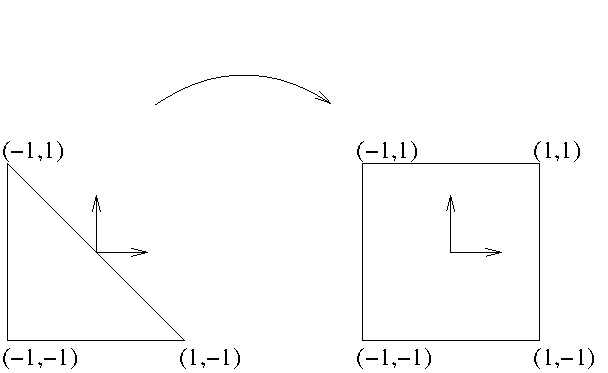
\includegraphics[height=6cm]{chapters/kirby-1/pdf/tricoord.pdf} 
\end{center}
\caption{Reference triangular and square domains with collapsed
  coordinate transformation.}
\label{fig:tricoord}
\end{figure}


While this basis is more complicated than the power basis, it is very
well-conditioned for numerical calculations even with high degree
polynomials.  The polynomials can also be ordered hierarchically so
that
\( \{ \psi_i \}_{i=1}^{n} \) forms a basis for $\P_{n-1}$ 
for each \( n > 1 \).  As a possible disadvantage, the
basis lacks rotational symmetry that can be found in  other bases.

\paragraph{Bernstein basis.}
The Bernstein basis is another well-conditioned basis that can be
used in generating finite element bases.
In 1D, the  basis functions in $\P_q$ take the form,
\begin{equation}
\psi_i^q = \binom{q}{i} x^i (1-x)^{q-i}, \quad i=0,\ldots,q,
\end{equation}
and then \( \P_q \) is spanned by \( \{ \psi_i^q \}_{i=0}^q \).

Notice that the Bernstein basis consists of powers of \( x \) and \( 1-x \),  which are the
barycentric coordinates for \( [0,1] \), an observation that makes it
easy to extend the basis to simplices in higher dimensions.
Let $b_1$, $b_2$, and $b_3$ be the barycentric coordinates for
the reference triangle; that is,
$b_1=1-x-y$, $b_2=x$, and $b_3=y$. Then the basis is
of the form,
\begin{equation}
\psi_{ijk}^q = \frac{q!}{i!j!k!} b_1^i b_2^j b_3^k, \quad  \mbox{for} \ i+j+k=q .
\end{equation}
and a basis for $\P_q$ is simply.
\begin{equation}
\{ \psi_{ijk}^q \}_{i,j,k\geq 0}^{i+j+k = q} .
\end{equation}
The Bernstein polynomials on the tetrahedron and even higher
dimensional simplices are completely analogous.

These polynomials, though less common in the finite element community,
are well-known in graphics and splines.  They have 
rotational symmetry and are nonnegative and so give positive
mass matrices, though they are not hierarchical.
Recently, \citet{Kirby2009,Kirby2010} has analyzed finite element operators based on Bernstein
polynomials.  In these papers, particular properties of the Bernstein
polynomials are exploited to develop algorithms for matrix-free
application of finite element operators with complexity comparable to
spectral elements.


\paragraph{Homogeneous polynomials.}
\label{sec:homo:pol}

Another set of polynomials which sometimes is useful is the set
of homogeneous polynomials $\H^q$. These are polynomials where all terms
have the same degree. $\H^q$ is in 2D spanned by polynomials on the
form:
\begin{equation}
\{ x^i y^j \}_{i+j=q} 
\end{equation}
with a similar definition in $d$D.



\paragraph{Vector or tensor valued polynomials.}
It is straightforward to generalize the scalar valued polynomials discussed
earlier to vector or tensor valued polynomials. Let $\{e_i\}$ be canonical
basis in $\R^d$. Then a basis for the vector valued polynomials is
\[
\phi_{ij} = \phi_j \mathbf{e}_i,
\]
with a similar definition extending the basis to tensors.


\section{Examples of elements}

We include some standard finite elements to illustrate the concepts. 
We refer the reader to Chapter~\ref{chap:kirby-7} for a more thorough review of
elements and their properties. 

\begin{figure}
  \begin{center}
    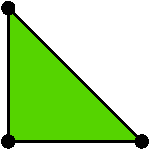
\includegraphics[height=3cm]{chapters/kirby-6/pdf/P1.pdf} \hspace{1.0cm}
    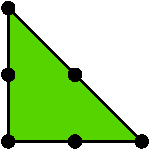
\includegraphics[height=3cm]{chapters/kirby-6/pdf/P2.pdf} \hspace{1.0cm}
%    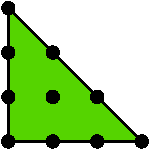
\includegraphics[height=3cm]{chapters/kirby-6/pdf/P3.pdf}
    \caption{Lagrange elements of order 1 and 2.}
    \label{Lagrange}
  \end{center}
\end{figure}

\begin{example}{\bf{The Lagrange Element}} \\
The Lagrange element shown in Figure \ref{Lagrange} is the most common element.
The degrees of freedom are represented by black dots, which represent point evaluation. 
The first order element is shown in the leftmost triangle, 
its degrees of freedom consist of a point evaluation in each of the vertices. 
That is, the degrees of freedom $\ell_i : \mathcal{V} \rightarrow \mathbb{R}$ are  
\begin{equation}
\ell_i ( v) = \int_{T} v \, \delta_{x_i} \, dx = v(x_i),   
\end{equation}
where $x_i$ are the vertices (0,0), (1,0), (0,1).
The corresponding basis functions
are $1-x-y$, $x$, and $y$.  The second order element is shown in right 
triangle. It has six degrees of freedom, three at the vertices and three
at the edges, all are point evaluations.  
The Lagrange element produces piecewise continuous polynomials and they are therefore
well suited for approximation in $H^1$.
The Lagrange element of order $q$ spans $\P_q$ on simplices in any dimension.  
\end{example}

\begin{figure}
  \begin{center}
    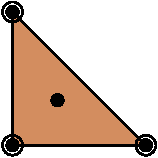
\includegraphics[height=3cm]{chapters/kirby-6/pdf/HER3.pdf}
    \caption{Hermite elements of order 3.}
    \label{Hermite}
  \end{center}
\end{figure}

\begin{example}{\bf{ The Hermite Element}} \\
In Figure \ref{Hermite} we show the Hermite element on the reference triangle in 2D. The black dots mean point
evaluation, while the white circles mean evaluation of derivatives in both $x$ and
$y$ direction. 
That is, the degrees of freedom $\ell_{i_k} : \mathcal{V} \rightarrow \mathbb{R}$ 
associated with the vertex $x_i$ are,  
\begin{eqnarray}
\ell_{i_1} ( v) &=& \int_{T} {v} \, \delta_{x_i} \, dx = v(x_i),    \\
\ell_{i_2} ( v) &=& \int_{T} \frac{\partial{v}}{\partial x} \, \delta_{x_i} \, dx = \frac{\partial}{\partial x} v(x_i),  \\  
\ell_{i_3} ( v) &=& \int_{T} \frac{\partial{v}}{\partial y} \, \delta_{x_i} \, dx = \frac{\partial}{\partial y} v(x_i) .    
\end{eqnarray}
In addition, there is one internal point evaluation, which in total gives ten degrees of freedom, which is the same number
of degrees of freedom as in $\P^2_3$.  One feature of the Hermite element
is that it has continuous derivatives at the vertices (it will however
not necessarily result in a $H^2$ conforming approximation).
\end{example}

\begin{figure}
  \begin{center}
    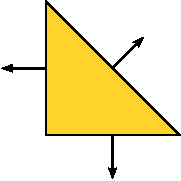
\includegraphics[height=3.5cm]{chapters/kirby-6/pdf/RT0.pdf} 
    \caption{Triangular Raviart--Thomas elements of order 0}
    \label{Raviart-Thomas}
  \end{center}
\end{figure}

\begin{example}{\bf{The Raviart--Thomas Element}} \\
In Figure \ref{Raviart-Thomas} we illustrate the lowest order Raviart--Thomas element.
In contrast to the previous elements, this element has a vector-valued
function space.  The arrows represent normal vector; that is, the 
degrees of freedom $\ell_i : \mathcal{V} \rightarrow \mathbb{R}$ are  
\begin{equation}
\ell_i ( v) = \int_{T} v \cdot n_i  \, dx ,  
\end{equation}
where $n_i$ is the outward normal vector on edge $i$.
The Raviart--Thomas element is a vector space with three degrees of freedom. Hence, 
the standard basis $\P^d_q$ is not a suitable starting point and we use 
$\mathcal{V} = \P_0^2 \oplus x \H_0$ instead.   
The Raviart--Thomas element is typically used for approximations in $\Hdiv$.
We remark that this element may also be defined in terms of point evaluations of normal components.
\end{example}

%\begin{remark}
%Earlier we saw common bases for $\P^n_d$, but
%elements like the Raviart--Thomas element described above use function
%spaces other than \( \P^n_d \) or vectors or tensors thereof.  To fix
%this, we must either construct a basis for the appropriate polynomial
%space or work with a different element that includes full vectors of
%$\P^n_d$.  In the case of \( H(\mathrm{div}) \) elements, this
%corresponds to using the Brezzi-Douglas-Fortin-Marini elements.
%\end{remark}
%

\subsection{Bases for other polynomial spaces}
The basis presented above are suitable for constructing many finite
elements, but as we have just seen, they do not work in all cases.
The Raviart-Thomas function space in 2D is spanned by
\[
\left( \P^2_n \right)^2 \oplus
\left(\begin{array}{c} x \\y \end{array} \right) \, \H^2_n, 
\]
Hence, this element requires a basis for vectors of polynomials  $(\P^2_n)^2$  enriched with 
$ \left(\begin{array}{c} x \\y \end{array} \right)  \, \H^2_n$.
On the other hand,  the Brezzi-Douglas-Fortin-Marini on triangle is defined as  
\begin{equation}
\left\{
u \in (\P^2_n (T) )^2 : u \cdot n \in \P^1_{n-1}(\gamma), \gamma \in \mathcal{E}(T)
\right\}.
\end{equation}
Hence, this element requires that some functions are removed from   
$\P^2_n (T)$. The removal is expressed by the constraint  $u \cdot n \in \P^1_{n-1}(\gamma)$.

Obtaining a basis for this space is somewhat more subtle.  
FIAT and SyFi have developed different
but mathematically equivalent solutions.  
In SyFi, since it uses a symbolic representation, the polynomial may be easily expressed 
in the power basis and the coefficients corresponding to second order polynomials 
normal to the edges are set to zero. In a similar fashion, FIAT utilizes the orthogonality of the Legendre polynomials  
 to express the constraints the edges. That is, on the edges $E_i$ the functionals (or constraints)    
\[
\ell^C_i( u ) = \int_{E_i} (u \cdot n) \mu_n^i = 0,  
\]
where $\mu_n^i$ is the second order Legendre polynomial on the edge $E_i$.  


In general, assume that we have $m$ constraints and $n-m$ degrees of freedom.
Let 
\begin{eqnarray}
V^1_{ij} &=& \ell_i( \phi_j ), \quad  1\le i \le n-m, \  1\le j \le n,  \\
V^2_{ij} &=& \ell^C_i( \phi_j ), \quad  n-m  < i \le n, \  1\le j \le n, 
\end{eqnarray}
Then,
\begin{equation}
V = \left( \begin{array}{c} V^1 \\ V^2 \end{array} \right).
\end{equation}
Here, \( V^1 \in \mathbb{R}^{n-m, n} \) and
\( V^2 \in \mathbb{R}^{m, n} \) are defined
by
\[V^1_{ij} = \ell_i( \phi_j ),
\]
\[
V^2_{ij} = \ell^C_i( \phi_j ),
\]
where \( \{ \phi_j \}_{j=1}^{2 \kappa} \) is a basis for \( (\P^2_n)^2
\).

Consider now the matrix
equation
\begin{equation}
\label{eq:extendedvdmsystem}
V A^t = I^{n,n-m},
\end{equation}
where \( I^{n,n-m} \) denotes the \( n \times n-m \) identity matrix.  
As before, the columns of \( A \) still
contain the expansion coefficients of the nodal basis functions
\( \psi_i \) in terms of \( \{ \phi_j \} \).
Moreover, \( V_2 A = 0 \), which implies that the nodal basis functions
fulfill the constraint. 

Other examples than the Brezzi-Douglas-Fortin-Marini element 
that are defined in terms of constrained polynomials are 
\nedelec~\citep{Nedelec1980}, Arnold-Winther~\citep{ArnoldWinther2002},
Mardal-Tai-Winther~\citep{MardalTaiWinther2002}, 
Tai-Winther~\citep{TaiWinther2006}, and Bell~\citep{Ciarlet2002} element families.


\section{Operations on the polynomial spaces}
Here, we show how various important operations may be cast
in terms of linear algebra operations, supposing that the operations may be performed on
the original basis \( \{ \psi_i \}_{i=1}^{n} \).

\subsection{Evaluation}
In order to evaluate the nodal basis \( \{ \phi_i \}_{i=1}^{n} \)
at a given point \( x \in T \), one simply computes the vector
\begin{equation}
\Psi_i = \psi_i(x)
\end{equation}
followed by the product
\begin{equation}
\phi_i(x) \equiv \Phi_i = \alpha_{ij} \Psi_j.
\end{equation}
Generally, the nodal basis functions are required at an array of
points \( \{ x_j \}_{j=1}^{m} \subset T \).  For performance reasons,
performing matrix-matrix products may be advantageous.  So, define
\( \Psi_{ij} = \Psi_i(x_j) \)  and \( \Phi_{ij} = \Phi_i(x_j) \).
Then all of the nodal basis functions may be evaluated by the
product
\begin{equation}
\Phi_{ij} = \alpha_{ik} \Psi_{kj}.
\end{equation}
\subsection{Differentiation}
Differentiation is more complicated and presents more options.
Let \( \alpha = ( \alpha_1 , \alpha_2 , \dots \alpha_d ) \) be a
multi-index so that
\begin{equation}
D^\alpha \equiv \frac{\partial^{|\alpha|}}{\partial
  x_1^{\alpha_1} \partial x_2^{\alpha_2} \dots \partial x_d^{\alpha_d}},
\end{equation}
where \( |\alpha| = \sum_{i=1}^{d} \alpha_i \) and we want 
to compute the array
\begin{equation}
\Phi^\alpha_i = D^\alpha \phi_i(x)
\end{equation}
for some \( x \in T \).

One obvious option is to differentiate the
original basis functions \( \{ \psi_i \} \) to produce an array
\begin{equation}
\Psi^\alpha_i = D^\alpha \psi_i(x),
\end{equation}
whence
\begin{equation}
\Phi^\alpha_i = \alpha_{ij} \Psi^\alpha_i.
\end{equation}
This presupposes that one may conveniently compute all derivatives of
the \( \{ \psi_i \} \).  This is typically true in symbolic
computation or when using the the power basis.  
For the Bernstein, Jacobi, and Legendre
 polynomials recurrence relations are
available, see \citep{KarniadakisSherwin2005,Kirby2010}.  
The Dubiner basis, as typically formulated, contains a coordinate
singularity that prevents automatic differentiation from working at
the top vertex.  Recent work by \citet{Kirby} has reformulated recurrence
relations to allow for this possibility.

If one prefers (or is required by the particular starting basis), one
may also compute matrices that encode first derivatives acting on the
\( \{ \phi_i \} \) and construct higher derivatives than these.
For each coordinate direction \( x_k \), a matrix \( \mathrm{D}^k \)
is constructed so that
\begin{equation}
\frac{\partial \phi_i}{\partial x_i} =
D^k_{ij} \phi_j.
\end{equation}
How to do this depends on which bases are chosen.  For particular
details on the Dubiner basis, see~\citep{Dubiner1991}.  
%Then, \( \Psi^\alpha \)
%may be computed by
%\[
%\Psi^\alpha_i = (\mathrm{D}^\alpha A)_{ij} \Phi_{j},
%\]

\subsection{Integration}
Integration of basis functions over the reference domain, including products of
basis functions and/or their derivatives, may be performed numerically,
symbolically, or exactly with some known formula. 
In general, quadrature is easily performed. 
Quadrature rules for a variety of reference elements may 
be obtained from for example \citep{Dunavant1985,KeeganRidzalBochev2008,SolinSegethDolevzel2004}.

%If Bernstein polynomials are used, we may use the formula
%\[
%\int_K b_1^i b_2^j b_3^k \, dx = \frac{i!j!k!}{(i+j+k+2)!}\frac{|K|}{2}
%\]
%on triangles and a similar formula for lines and tetrahedra
%to calculate integrals of expressions containing these terms exactly.  Alternately, if the Dubiner basis is used,
%orthogonality may be used.  In either case, when derivatives occur, it
%may be as efficient to use numerical quadrature.  On rectangular
%domains, tensor products of Gauss or Gauss-Lobatto quadrature can be
%used to give quadrature families to any order accuracy, although
%in some cases so-called sparse rules may win~\citep{KeeganRidzalBochev2008}
%On the simplex, efficient quadrature is more difficult to find.
%Rules based on barycentric symmetry~\citep{Dunavant1985} may be used up to a
%certain degree (which is frequently high enough in practice).  If one
%needs to go beyond these rules, it is possible to use the
%mapping~(\ref{eq:dubcoord}) to map tensor products of Gauss-Jacobi
%quadrature rules from the square to the triangle.

\subsection{Association with facets}
As we saw in the definition of for instance the  Brezzi-Douglas-Marini element,  
it is necessary to have polynomials that can be associated with the facets of a polygonal 
domain. The Bernstein polynomials are expressed via barycentric coordinates
and are therefore naturally associated with the facets. The Legendre and Jacobi polynomials are
also easy to associated to 1D facets in barycentric coordinates.  


\subsection{Linear functionals}
Linear functionals are usually cast in terms of linear combinations of integration, pointwise evaluation and differentiation. 

\subsection{The mapping of the reference element}

A common practice, employed throughout the FEniCS
software and in many other finite element codes, is to map the nodal
basis functions from the reference cell to each cell in a mesh.
Sometimes, this is as simple as an affine change of coordinates; in
other cases it is more complicated.
For completeness, we briefly describe the basics of creating the global finite elements in terms of a mapped
reference element. Let therefore $T$ be a global polygon in the mesh and $\hat{T}$ be the corresponding reference polygon.
Between the coordinates
$x\in T$ and $\hat x\in\hat T$ we use the mapping
\begin{equation}
\label{eq:geometry}
x = F_T(\hat x) = A_T(\hat x)  + x_0,
\end{equation}
The Jacobian of this mapping is: 
\begin{equation}
\label{eq:geometry2}
J(\hat x) =  \frac{\partial x }{\partial \hat x}  =    \frac{\partial A_T(\hat x) }{\partial \hat x} .
\end{equation}
Currently, FEniCS only supports affine maps between $T$ and $\hat{T}$, which means that 
$x = F_T(\hat x) = A_T\hat x  + x_0$ and $J=A_T$.
For isoparametric elements, a basis function is defined in terms of the corresponding basis function
on the reference element as
\begin{equation}
\label{eq:subs}
\phi(x) = \hat{\phi}(\hat x). 
\end{equation}
The integral can then be performed on the reference polygon,
\begin{equation}
\label{eq:integration2}
\int_T \, \phi (x) \, dx = \int_{\hat{T}} \, \hat \phi (\hat x) \, detJ d\hat x ,
\end{equation}
and the spatial derivatives are defined by the derivatives on the
reference element and the geometry mapping by using the
chain rule,
\begin{equation}
\label{eq:chain}
\frac{\partial \phi}{\partial x_i} =
\sum_j \frac{\partial \hat \phi}{\partial \hat x_j} \frac{\partial \hat x_j }{\partial x_i }  .
\end{equation}

The above mapping of basis functions is common for approximations in $H^1$. For approximations in $\Hdiv$ or
$\Hcurl$ it is necessary to use the Piola mapping, where the mapping for the basis functions
differs from the geometry mapping. That is, for $\Hdiv$ elements, the Piola mapping reads  
\begin{equation}
\label{eq:subs}
\phi(x) = \frac{1}{|detJ|} J \hat{\phi}(\hat x),
\end{equation}
When using the numbering of mesh entities used by UFC, see Chapter~\ref{chap:alnes-2}, it is advantageous to use $\frac{1}{detJ}$ instead of $\frac{1}{|detJ|}$ since the sign of the determinant relates to the sign of the normal vector,     
see ~\citep{RognesKirbyLogg2009} for more details on the Piola mapping and its implementation in FFC.   
Some elements like the Rannacher-Turek element~\citep{Turek1999,RannacherTurek1992} has far better
properties when defined globally compared its analogous definition in terms
of a reference element.


\subsection{Local to global mapping of degrees of freedom}

As shown in Figure~\ref{fig:kirby-1:patch}, finite elements 
are patched together with a continuity depending on the degrees of freedom.  
To obtain the desired patching, the elements should provide identifiers that determining whether the degrees
of freedom of some neighboring elements should be shared or not.  
One alternative is to relate each degree of freedom on the reference cell to a point in the
reference cell. The geometry mapping then gives a global point in the mesh, by \eqref{eq:geometry}, that identifies the degree of freedom,
that is, the  degrees of freedom in different elements are shared if they correspond to the same global point in the mesh. 
Alternatively, each degree of freedom may be related to a local mesh entity, like a vertex, edge or face, on the reference element. After mapping the element, the degree of freedom will then be related to the corresponding mesh entity in the global mesh. This alternative requires that the corresponding mesh entities are numbered.      


\begin{figure}
  \begin{center}
%    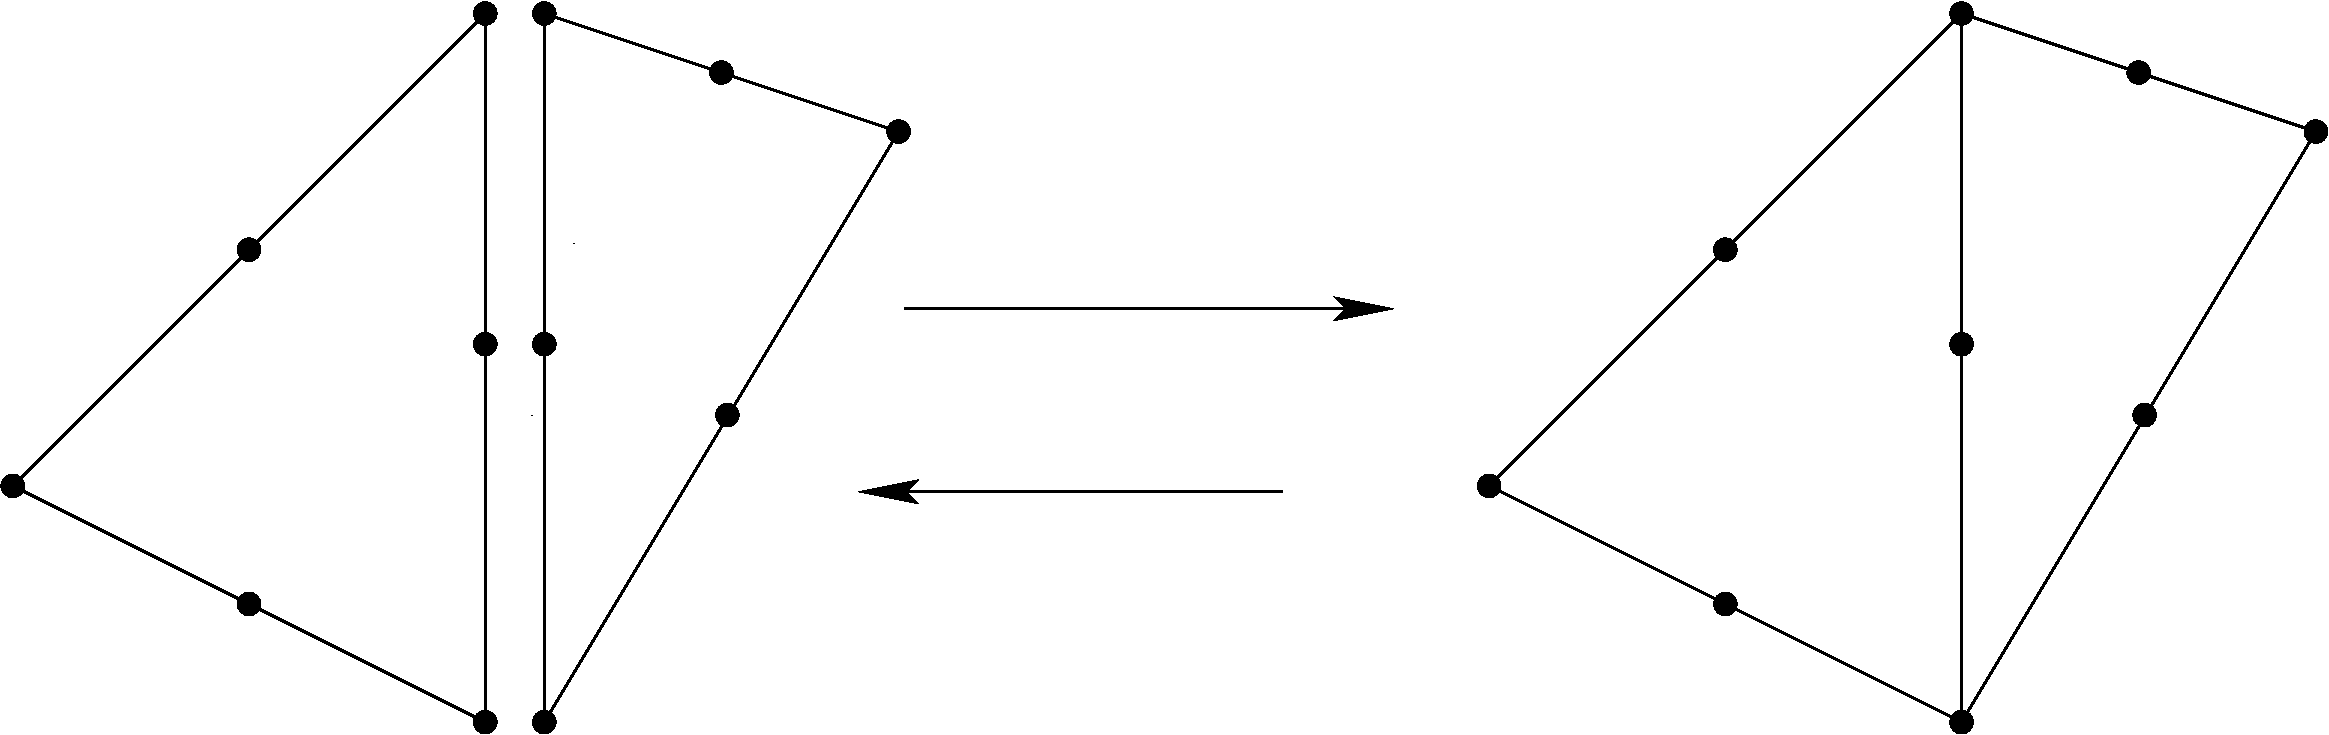
\includegraphics[width=\largefig]{chapters/kirby-1/pdf/patch.pdf}
    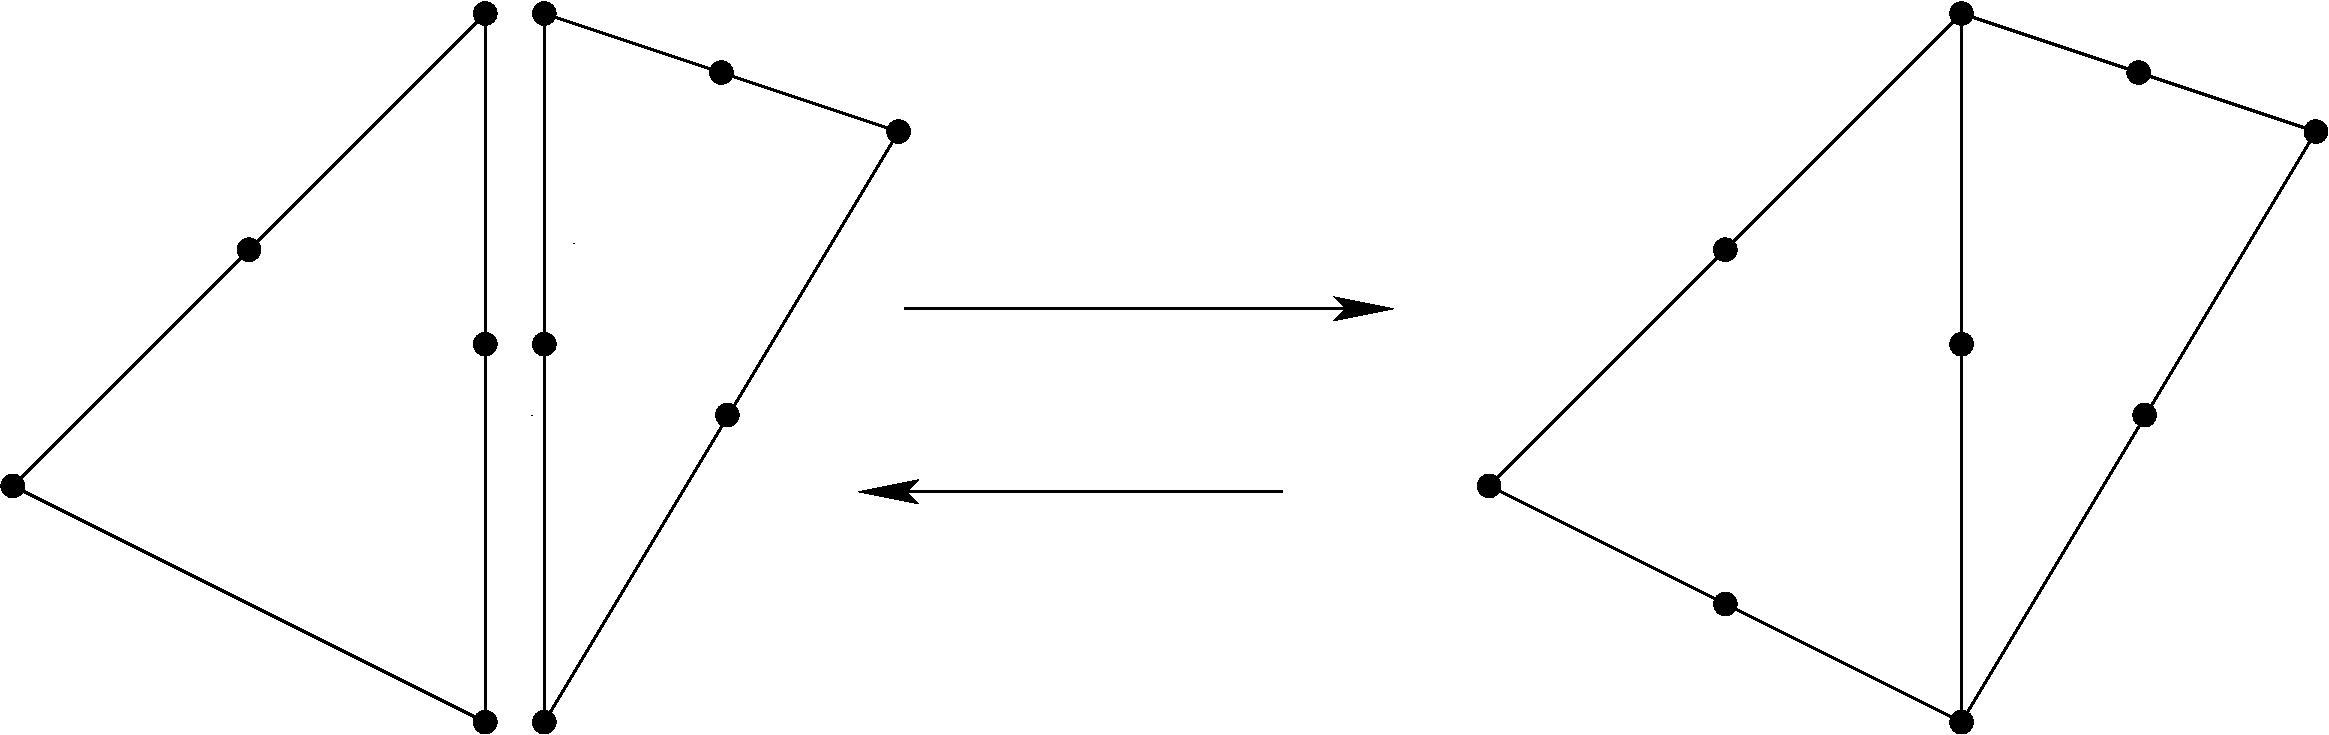
\includegraphics[width=\largefig]{unfinished/kirby-1/pdf/patch.pdf}
    \caption{Patching together a pair of quadratic local function
      spaces on a pair of cells to form a global continuous
      piecewise quadratic function space.}
    \label{fig:kirby-1:patch}
  \end{center}
\end{figure}


